Fora o navio (e os componentes que fazem parte dele, como mastro, escadas, etc), também foram produzidos dois objetos a parte: um timão e um telégrafo.

O timão e o telégrafo são apresentados na figura \ref{fig:tim_te}. O primeiro andar conta com duas salas. A figura \ref{fig:sala1} apresenta a primeira sala, enquanto a figura \ref{fig:sala2} apresenta a segunda. Na figura \ref{fig:niquel}, temos a sala do segundo andar renderizada. Nessas imagens, são apresentados alguns componentes que obtivemos prontos, como a mesa de sinuca, sofá e caça-níquel.

\begin{figure}[!h]
    \centering
    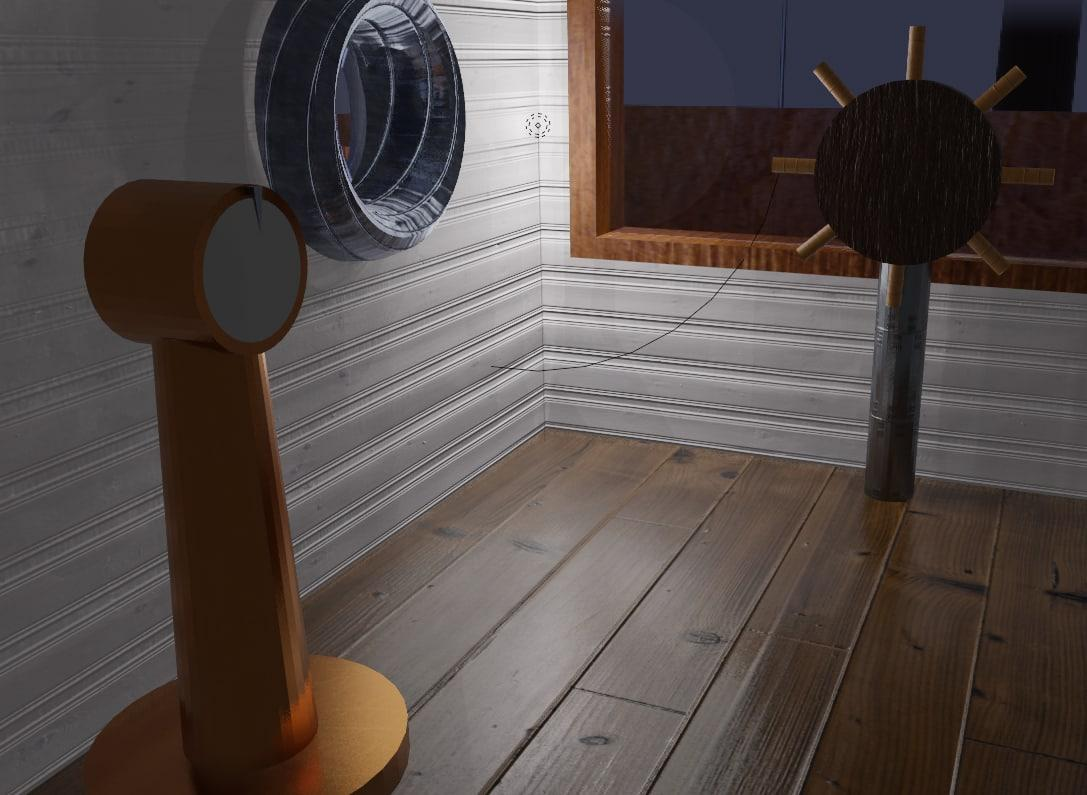
\includegraphics[scale=0.5]{imagens/timaotelegrafo.jpg}
    \caption{Timão e telégrafo renderizados.}
    \label{fig:tim_te}
\end{figure}

\begin{figure}[!h]
    \centering
    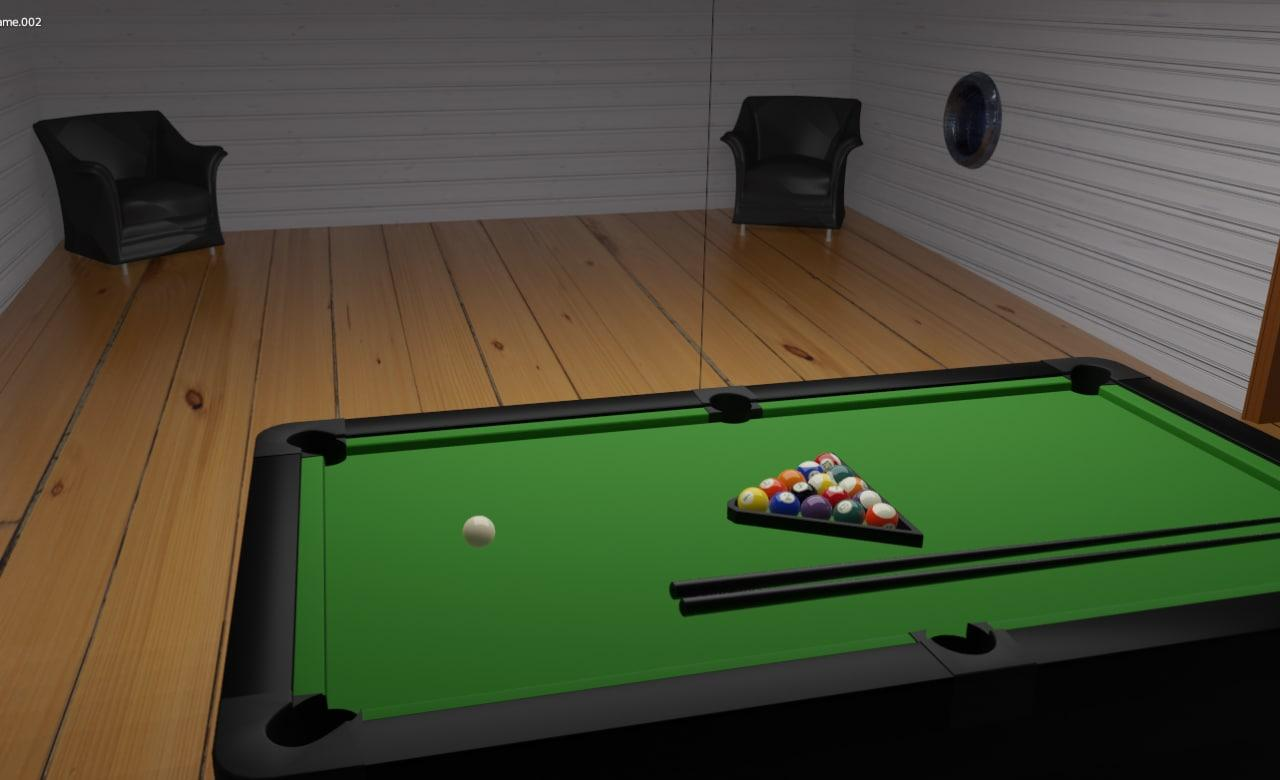
\includegraphics[scale=0.4]{imagens/sala1.jpg}
    \caption{Primeira sala do primeiro andar renderizada.}
    \label{fig:sala1}
\end{figure}


\begin{figure}[!h]
    \centering
    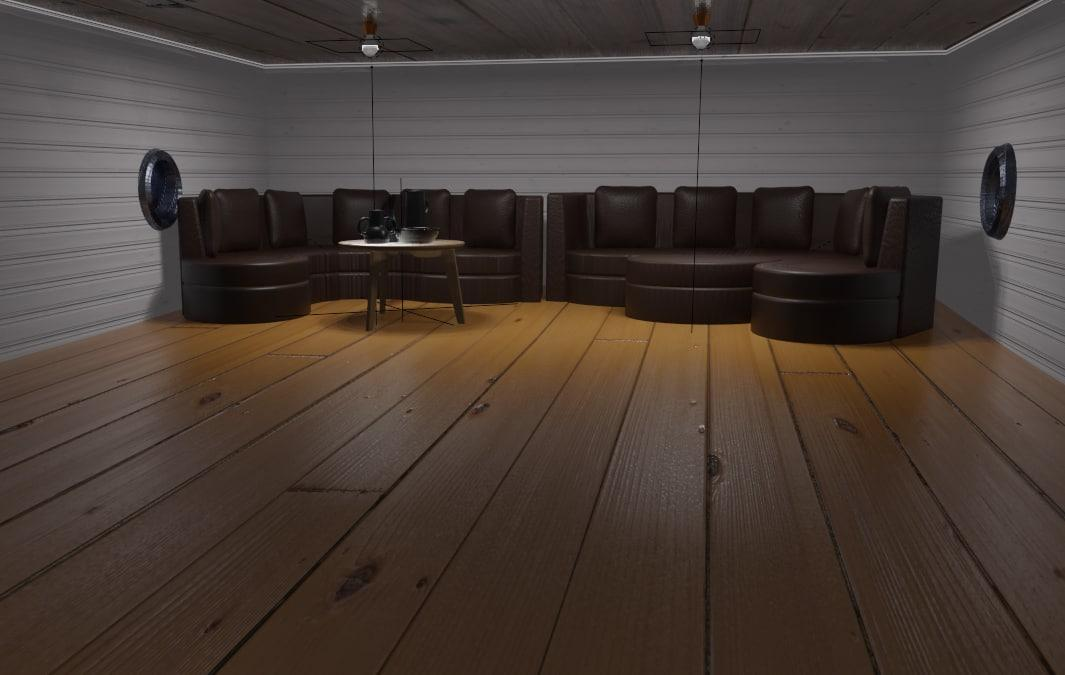
\includegraphics[scale=0.5]{imagens/sala2.jpg}
    \caption{Segunda sala do primeiro andar renderizada.}
    \label{fig:sala2}
\end{figure}


\begin{figure}[!h]
    \centering
    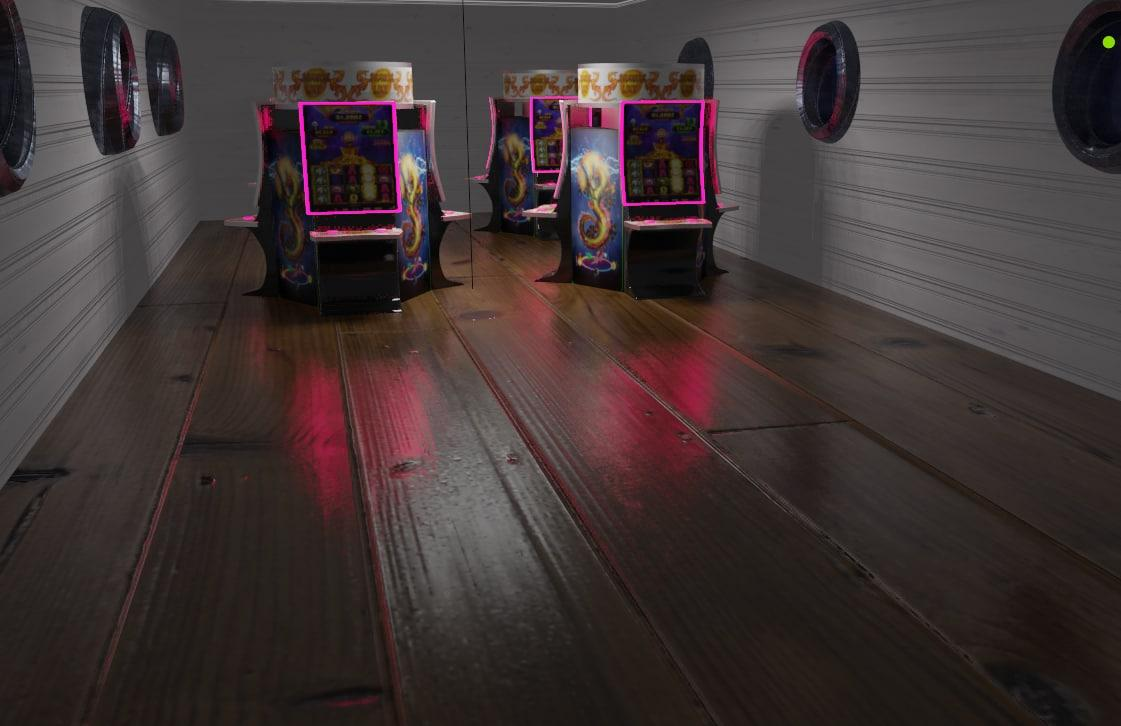
\includegraphics[scale=0.5]{imagens/sala.jpg}
    \caption{Sala do segundo andar renderizada.}
    \label{fig:niquel}
\end{figure}

As imagens \ref{fig:p1}, \ref{fig:p2}, \ref{fig:p3}, \ref{fig:p4}, \ref{fig:p5}, \ref{fig:p6}, \ref{fig:p7} e \ref{fig:p8} retratam um pouco do processo de desenvolvimento do projeto pelo grupo, desde as primeiras estruturas criadas até o início da aplicação das texturas.

\begin{figure}[!h]
    \centering
    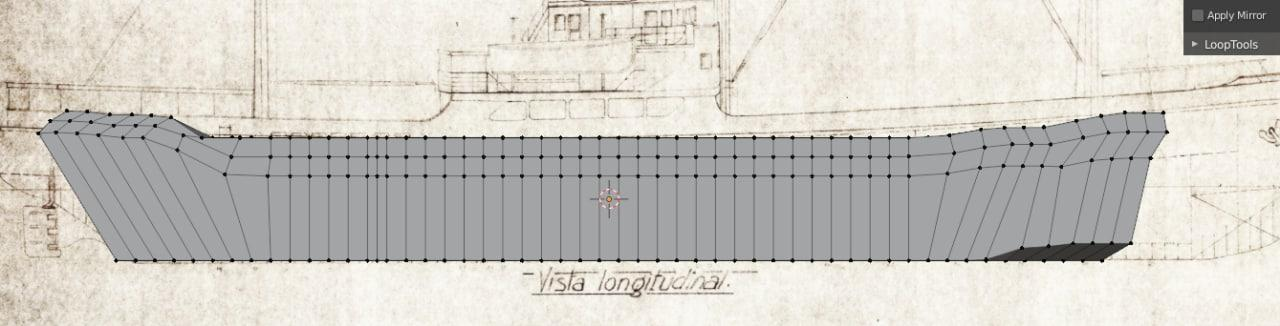
\includegraphics[scale=0.4]{imagens/p1.jpg}
    \caption{Processo de desenvolvimento.}
    \label{fig:p1}
\end{figure}

\begin{figure}[!h]
    \centering
    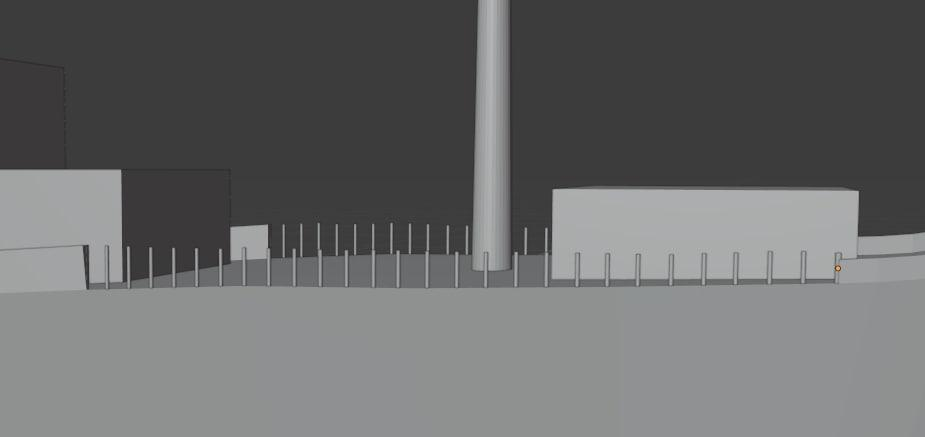
\includegraphics[scale=0.5]{imagens/p2.jpg}
    \caption{Processo de desenvolvimento.}
    \label{fig:p2}
\end{figure}

\begin{figure}[!h]
    \centering
    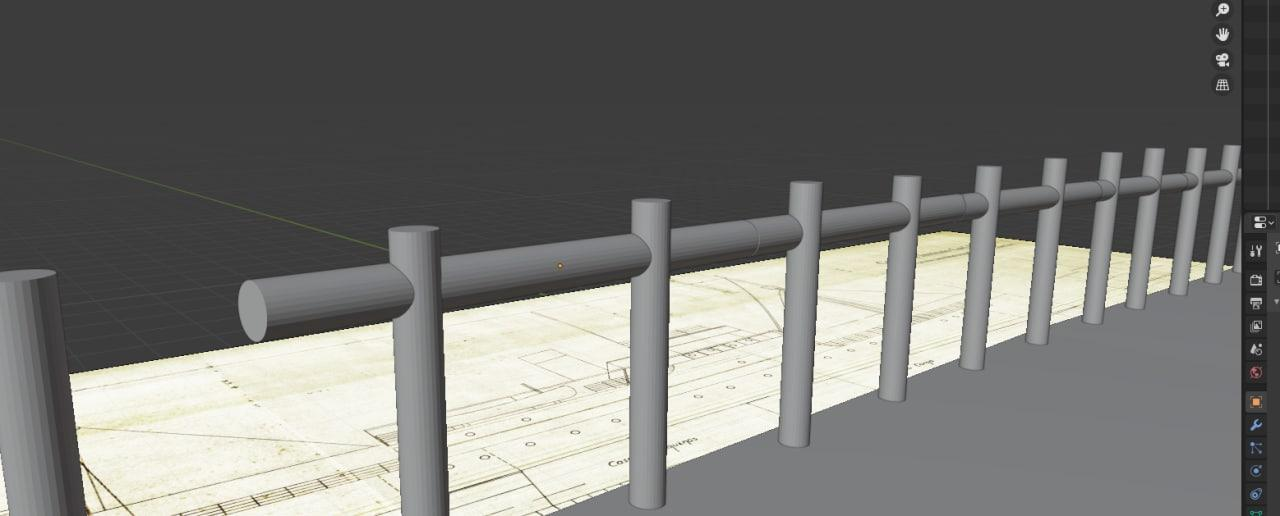
\includegraphics[scale=0.4]{imagens/p3.jpg}
    \caption{Processo de desenvolvimento.}
    \label{fig:p3}
\end{figure}

\begin{figure}[!h]
    \centering
    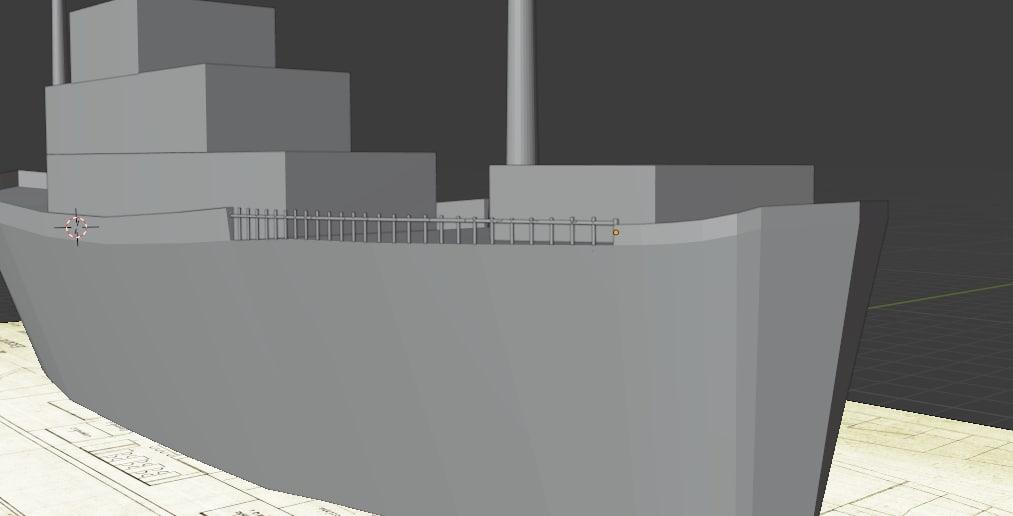
\includegraphics[scale=0.5]{imagens/p4.jpg}
    \caption{Processo de desenvolvimento.}
    \label{fig:p4}
\end{figure}

\begin{figure}[!h]
    \centering
    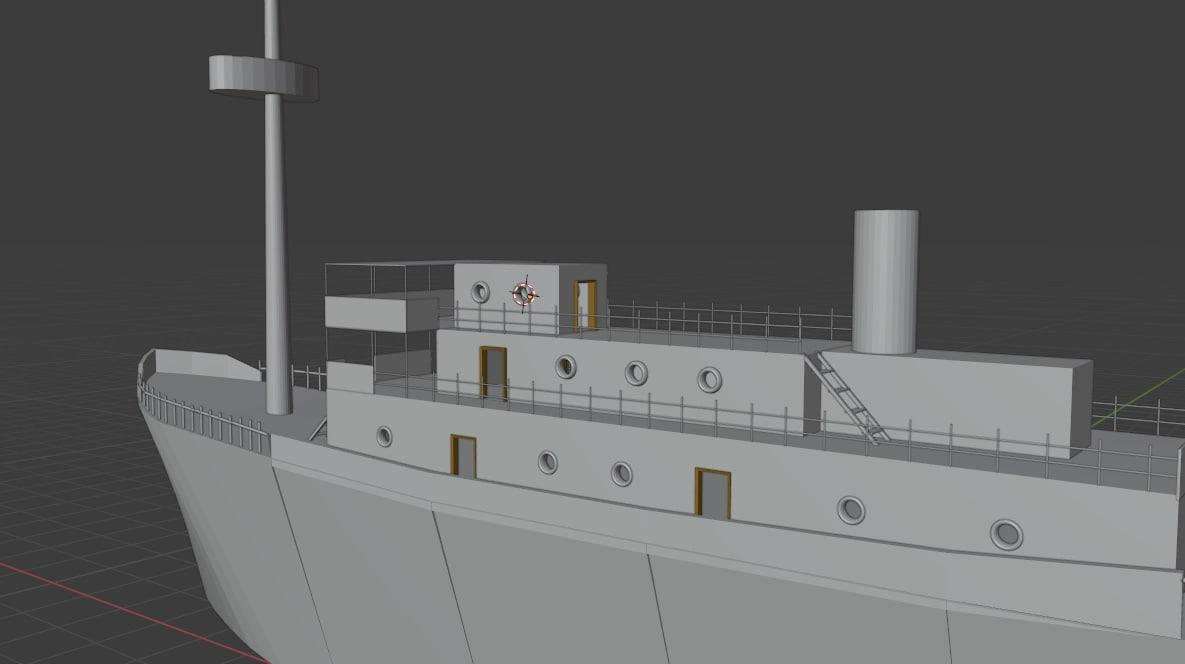
\includegraphics[scale=0.5]{imagens/p5.jpg}
    \caption{Processo de desenvolvimento.}
    \label{fig:p5}
\end{figure}

\begin{figure}[!h]
    \centering
    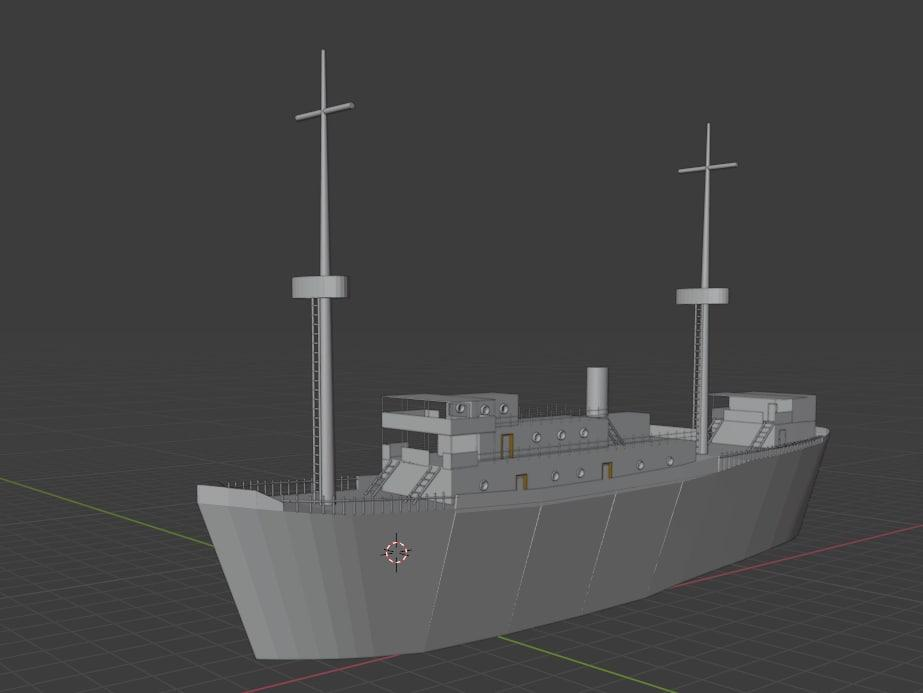
\includegraphics[scale=0.5]{imagens/p6.jpg}
    \caption{Processo de desenvolvimento.}
    \label{fig:p6}
\end{figure}

\begin{figure}[!h]
    \centering
    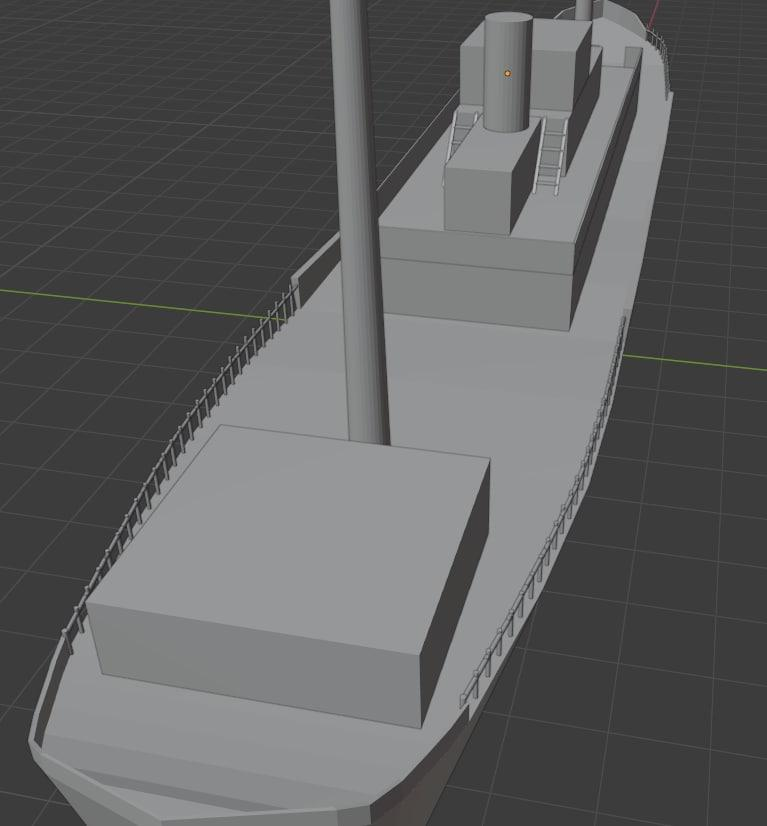
\includegraphics[scale=0.5]{imagens/p7.jpg}
    \caption{Processo de desenvolvimento.}
    \label{fig:p7}
\end{figure}

\begin{figure}[!h]
    \centering
    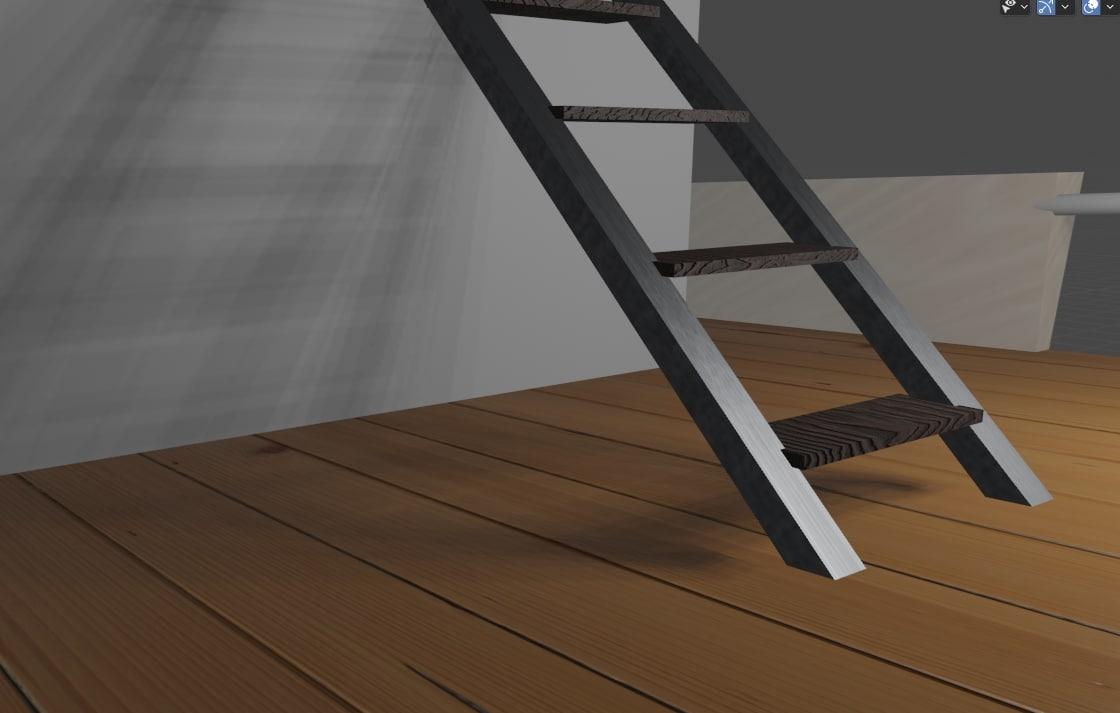
\includegraphics[scale=0.5]{imagens/p8.jpg}
    \caption{Processo de desenvolvimento.}
    \label{fig:p8}
\end{figure}

A figura \ref{fig:pf} apresenta o produto final do projeto, com as texturas aplicadas e o navio renderizado. Além dos arquivos do projeto, um vídeo será encaminhado junto a este relatório, realizando a visita virtual. Os vídeos renderizados para a visita foram feitos com a \textit{render engine} Eevee, enquanto as imagens renderizadas em alta qualidade foram feitas com a cycles utilizando 2000 amostras.  

\begin{figure}[!h]
    \centering
    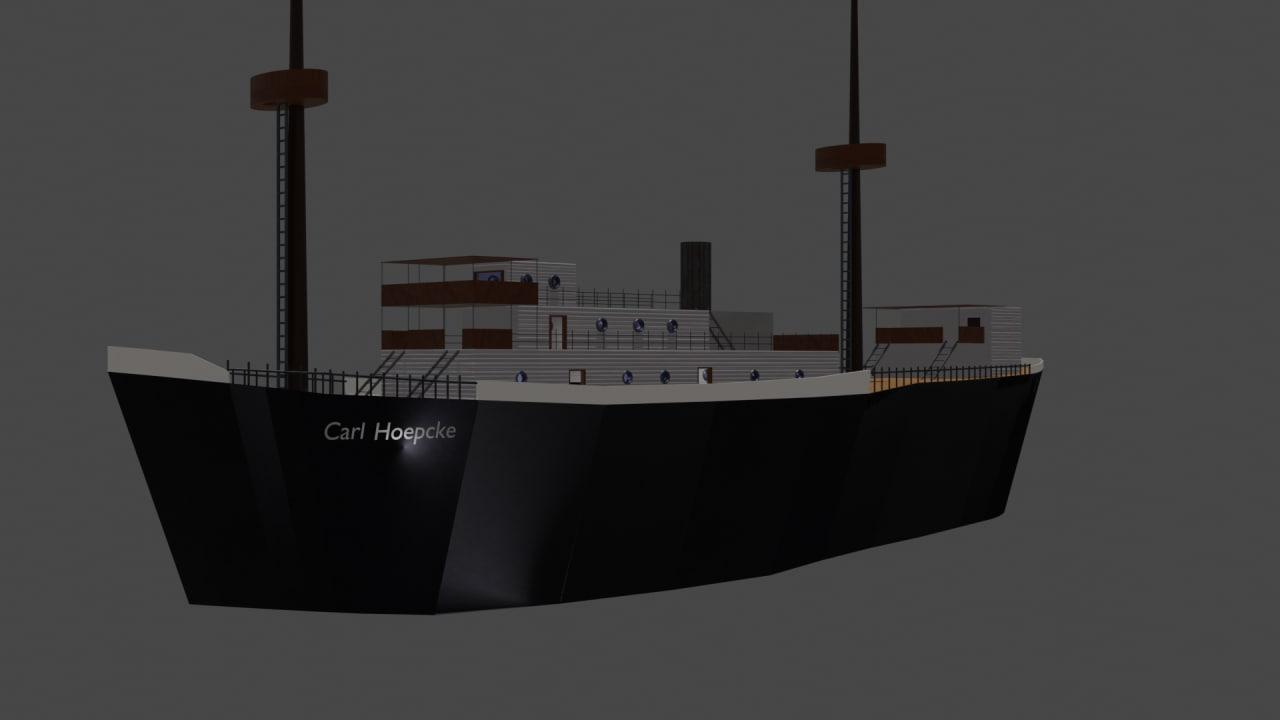
\includegraphics[scale=0.3]{imagens/render1.jpg}
    \caption{Produto final.}
    \label{fig:pf}
\end{figure}